\documentclass{article}
\usepackage[utf8]{inputenc}
\usepackage[T1]{polski}
\usepackage{classdiagram}


\usepackage[a4paper, margin=1.5cm]{geometry}
\usepackage{tikz}
\usetikzlibrary{calc}

\makeatletter
\def\firstauthor#1{\gdef\@firstauthor{#1}}
\def\@firstauthor{\@latex@warning@no@line{No \noexpand\firstauthor given}}
\def\projectname#1{\gdef\@projectname{#1}}
\def\@projectname{\@latex@warning@no@line{No \noexpand\projectname given}}
\newcommand\makeheader{%

\begin{tikzpicture}
    \node(IN){Imię i nazwisko};
    \node(IN1) at ($(IN) + (0, -0.5)$) {\@firstauthor};
\end{tikzpicture}
\vspace*{20pt}
\begin{center}
    
\begin{tikzpicture}
        \node(PN){\bf\LARGE\@projectname};
        \node(DOK) at ($(PN) + (0, 1)$) {\Large DOKUMENTACJA TECHNICZNA PROJEKTU};
        \node(PDM) at ($(PN) + (0, -1)$) {\Large Przedmiot: PROGRAMOWANIE OBIEKTOWE};
    \end{tikzpicture}
\end{center}
}
\makeatother


\projectname{System rozliczeń sztabu WOŚP, Java}
\firstauthor{Jan Chlebek}

\begin{document}

\makeheader

\section{Zakres projektu}
{\small\it Proszę wstawić kilkuzdaniowy opis projektu zawierający informacje:
\begin{enumerate}
    \item Do czego system będzie wykorzystywany?
    \\
    \textup{System stanowi uproszczoną symulację narzędzia do rozliczania puszek wykorzystywanych podczas WOŚP.}
    \item Jakie są granice używalności tworzonego systemu?
    \\
    \textup{System pozwala na zdefiniowanie dowolnego rodzaju waluty, która domyślnie nie jest uwzględniona w programie i posiada możliwość tworzenia lokalnych kopii zapasowych. Jego największym ograniczeniem jest działalność na maszynie lokalnej wyłącznie przez jednego użytkownika w danej chwili.}
    \item Jaki jest target systemu? (Do kogo system jest skierowany?)
    \\
    \textup{System skierowany jest dla administratorów sztabów WOŚP.}
    \item Z czego wynika potrzeba utworzenia systemu?
    \\
    \textup{Potrzeba wynika z chęci zrozumienia kompleksowości takich systemów i potrzeby inspiracji do rozbudowy obecnie wykorzystywanego na uczelni systemu sieciowego.}
\end{enumerate}}
\section{Diagram klas}
\textup{Ze względu na zaangażowanie czasowe w inne projekty diagram UML powstał w formie przybliżonej. Jego docelowa forma ulegnie poprawie i rozbudowaniu. Jeśli znacząco nie zwiększy się jego struktura, zostanie także przepisany do LaTeX.}

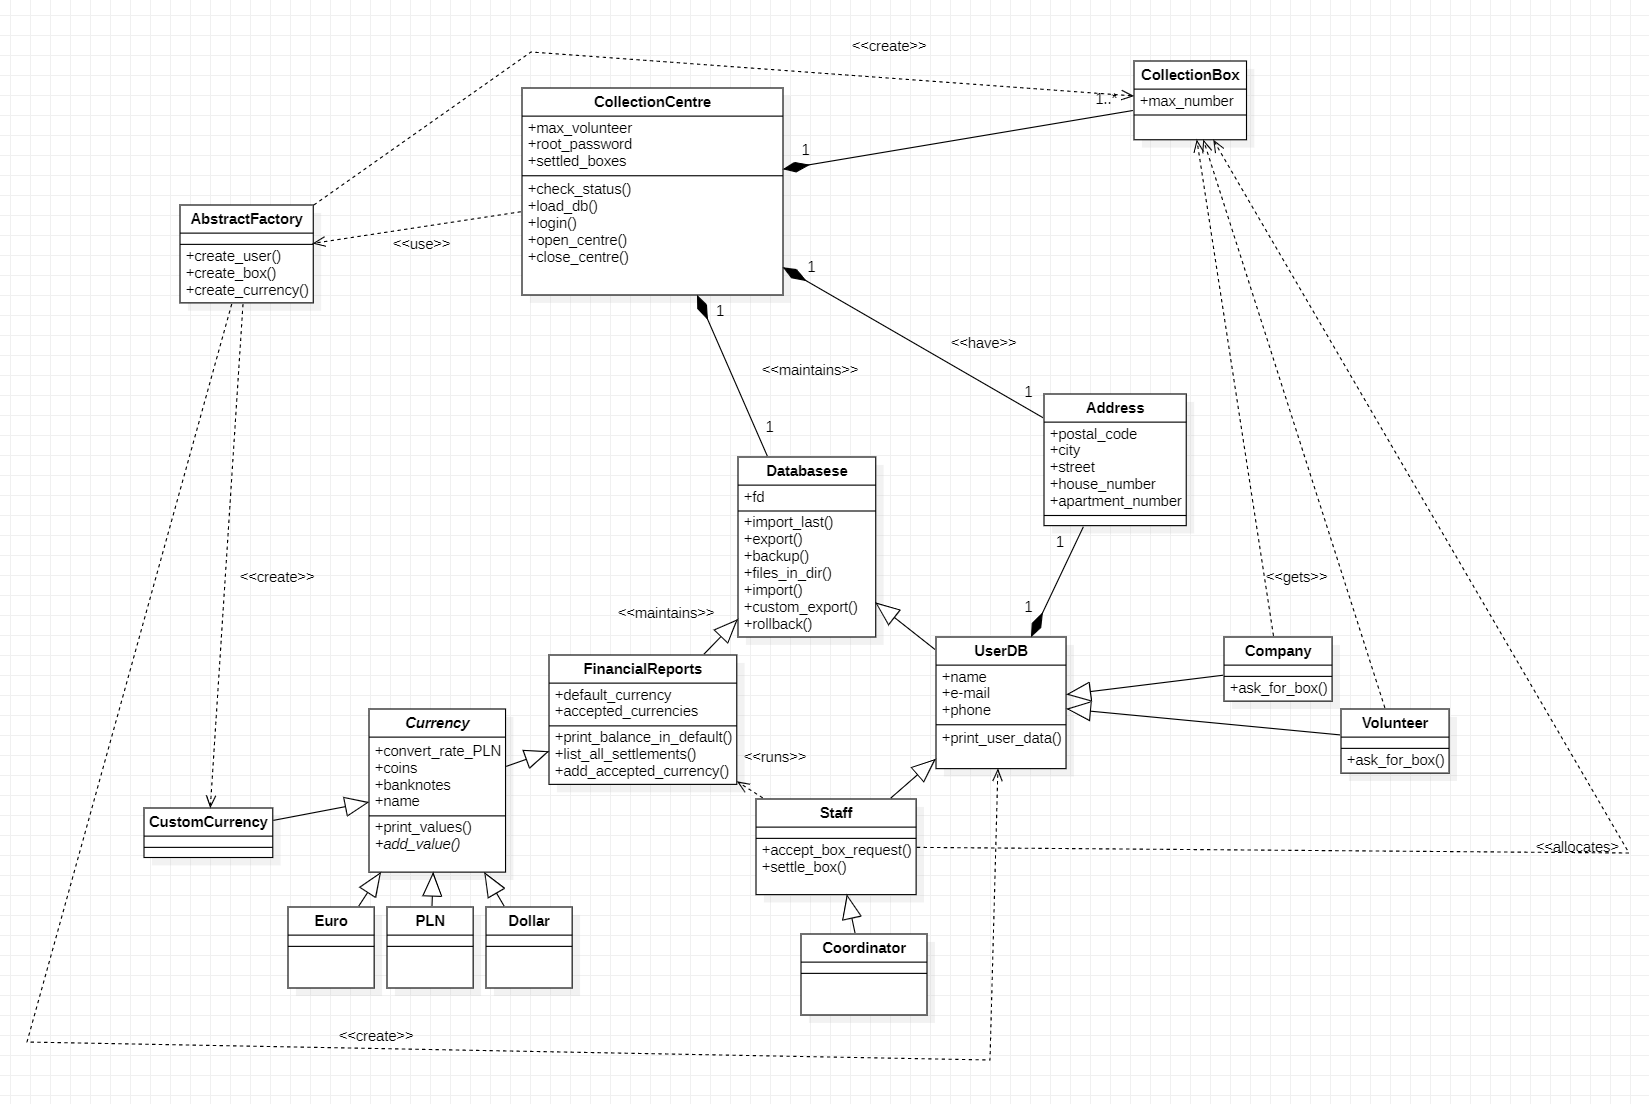
\includegraphics[width=\textwidth]{UML_v01.png}

\iffalse
  \begin{tikzpicture}[cd common/.append style={bottom color=white, top color=white},
                    cd package box/.append style={sharp corners, bottom color=white, top color=white},
                    cd package label/.append style={sharp corners, fill=white}]
  \begin{interface}{University} 
    \position{0, 0.5}
    \attribute[public]{score()}
    \operation[public]{getName() : String}
    \operation[protected]{getDean() : String}
    \operation[package]{getRector() : String}
  \end{interface}
  \begin{interface}{Student}
    \position[right=4cm]{University.east}
    \operation[public]{getFirstName(): String}
    \operation[protected]{getLastName(): String}
  \end{interface}
  \begin{class}{PUTStudent}
    \position[below left=1.0cm and 0.5cm]{Student.south}
    \operation[private]{getScholarship(): float}
    \operation[protected]{getMastersProgress(): float}
  \end{class}
  \begin{class}{ErasmusStudent}
    \position[below right=1.0cm and 0.5cm]{Student.south}
    \operation[public]{getNativeLanguage(): String}
    \operation[protected]{meet(Student): void}
  \end{class}
  \begin{class}{PUT}
    \position[below=1.0cm]{University.south}
    \operation[public]{getPrizes(): Prize[0..n]}
  \end{class}
  
  \generalization{PUT}{University}
  \generalization{PUTStudent}{Student}
  \generalization{ErasmusStudent}{Student}
  \aggregation{University}[students][0..*]{Student}
  \package{Example diagram}{(University)(Student)(PUT)(PUTStudent)(ErasmusStudent)}
\end{tikzpicture}
\fi

\section{Wymagania systemowe}
\subsection{Wymagania funkcjonalne}
{\small\it W tym miejscu powinno znaleźć się przynajmniej sześć funkcjonalności do zaimplementowania w projekcie z doperecyzowaniem w podpunktach.}
\begin{enumerate}
  \item Obsługa zapytań i przyznawania puszek
  \item Narzędzie rozliczania puszek w wielu walutach
  \item Export/Import lokalny danych
  \item Regularny backup podczas funkcjonowania systemu
  \item Możliwość obsługi terminala przez wielu użytkowników poprzez zmianę konta
  \item Narzędzia administracyjne z zabezpieczeniem hasłem programu
\end{enumerate}
\subsection{Wymagania pozafunkcjonalne}
{\small\it W tym miejscu powinny znaleźć się przynajmniej trzy wymagania pozafunkcjonalne narzucone na aplikację.}
\begin{enumerate}
  \item Wykorzystywanie wyłącznie standardowych bibliotek 
  \item Podawanie wartości pieniężnych z dokładnością do drugiego miejsca po przecinku
  \item Wieloplatformowość
\end{enumerate}
\section{Realizacja projektu}
{\small\it W tym miejscu proszę opisać procedurę, zgodnie z którą projekt będzie realizowany, np. jaka jest koncepcja zbioru bibliotek do wykorzystania przez system (ewentualnie kryteria zgodnie z którymi biblioteki będą wybierane), jakie jest wyobrażenie rytmu pracy nad projektem, jaki jest ramowy plan realizacji z wyszczególnieniem kroków milowych do celu utworzenia systemu.}
\\ \\
\textup{Projekt realizowany jest w sprintach skupiających się głównie na pojedynczych klasach, z wykorzystaniem wyłącznie domyślnych bibliotek języka. Ramowy plan zakłada najpierw realizację podstawowych funkcjonajlności niezbędnych do inicjalizacji sztabu, następnie przygotowania systemu rozliczeń i baz danych. Ze względu na zwinną metodykę działania, w późniejszym terminie przygotowany zostanie finalny diagram UML obrazujący pełną funkcjonalność programu.}
\section{Kryteria akceptacyjne}
\begin{enumerate}
  \item Wygenerowanie nowego Sztabu
  \item Wczytanie ostatniej bazy danych
  \item Testy odporności zaimplementowanych metod
  \item Audyt kodu
\end{enumerate}
\end{document}

